\PassOptionsToPackage{unicode}{hyperref}
\documentclass[9pt]{beamer}

\usetheme{TUDo}
\usefonttheme[onlymath]{serif}

\usepackage{fixltx2e}

% Sprachumgebung
\usepackage{polyglossia}
\setmainlanguage{german}

% Mathematik
\usepackage{amsmath}
\usepackage{amssymb}
\usepackage{mathtools}
\usepackage{cancel}
\usepackage[output-decimal-marker={,}]{siunitx}
\usepackage{tikz}

\usepackage{verbatim}

\usepackage[
  math-style=ISO,
  bold-style=ISO,
  sans-style=italic,
  nabla=upright,
  partial=upright,
]{unicode-math}
\setmathfont{Latin Modern Math}

\usepackage{fontspec}
\setsansfont{TeX Gyre Heros}

%Links
\usepackage{hyperref}
\usepackage{bookmark}

%%%%%%%%%%%%%%%%%%%%%%%%%%%%%%%%%%%%%%%%%%%%%%%%%%%%%%%%%%%%%%%%%%%%%%%%%%%%%%%%
%%%%%-------------Hier Titel/Autor/Grafik/Lehrstuhl eintragen--------------%%%%%
%%%%%%%%%%%%%%%%%%%%%%%%%%%%%%%%%%%%%%%%%%%%%%%%%%%%%%%%%%%%%%%%%%%%%%%%%%%%%%%%

%Titel:
\title{{\Huge Arduino}\\ \vspace{0.5cm} \textcolor{black}{Temperaturmesser\\ \\Leonard Wollenberg}}
%Autor
\author{Leonard Wollenberg}
%Lehrstuhl/Fakultät
\institute{Praktikum}
%Titelgrafik 
%\titlegraphic{Bilder/P2VV.pdf}


\begin{document}

	\begin{frame}
	  \setcounter{framenumber}{0}
	  \titlepage
	\end{frame}
	
	\begin{frame}
		\frametitle{Ziel}
		\begin{itemize}
				\item einen Thermometer zu bauen
				\item Ausgabe mit mehreren LEDs
				\item Messbereich $T\in[0,40)^\circ C$
		\end{itemize}
	\end{frame}

	\begin{frame}
		\frametitle{Umsetzung}
		\begin{itemize}
			\item Messung:  \textrm{TM36}
			\item Ausgabe: 8 Gelbe LEDs 2 rote LEDs 1 mehrfarbige LED
			\item Die Mehrfarbige LED zeigt die Zehner stelle
			\item Die einfarbigen LEDs zeigen die einer Stellen
		\end{itemize}
	\end{frame}

	\begin{frame}
		\begin{figure}
			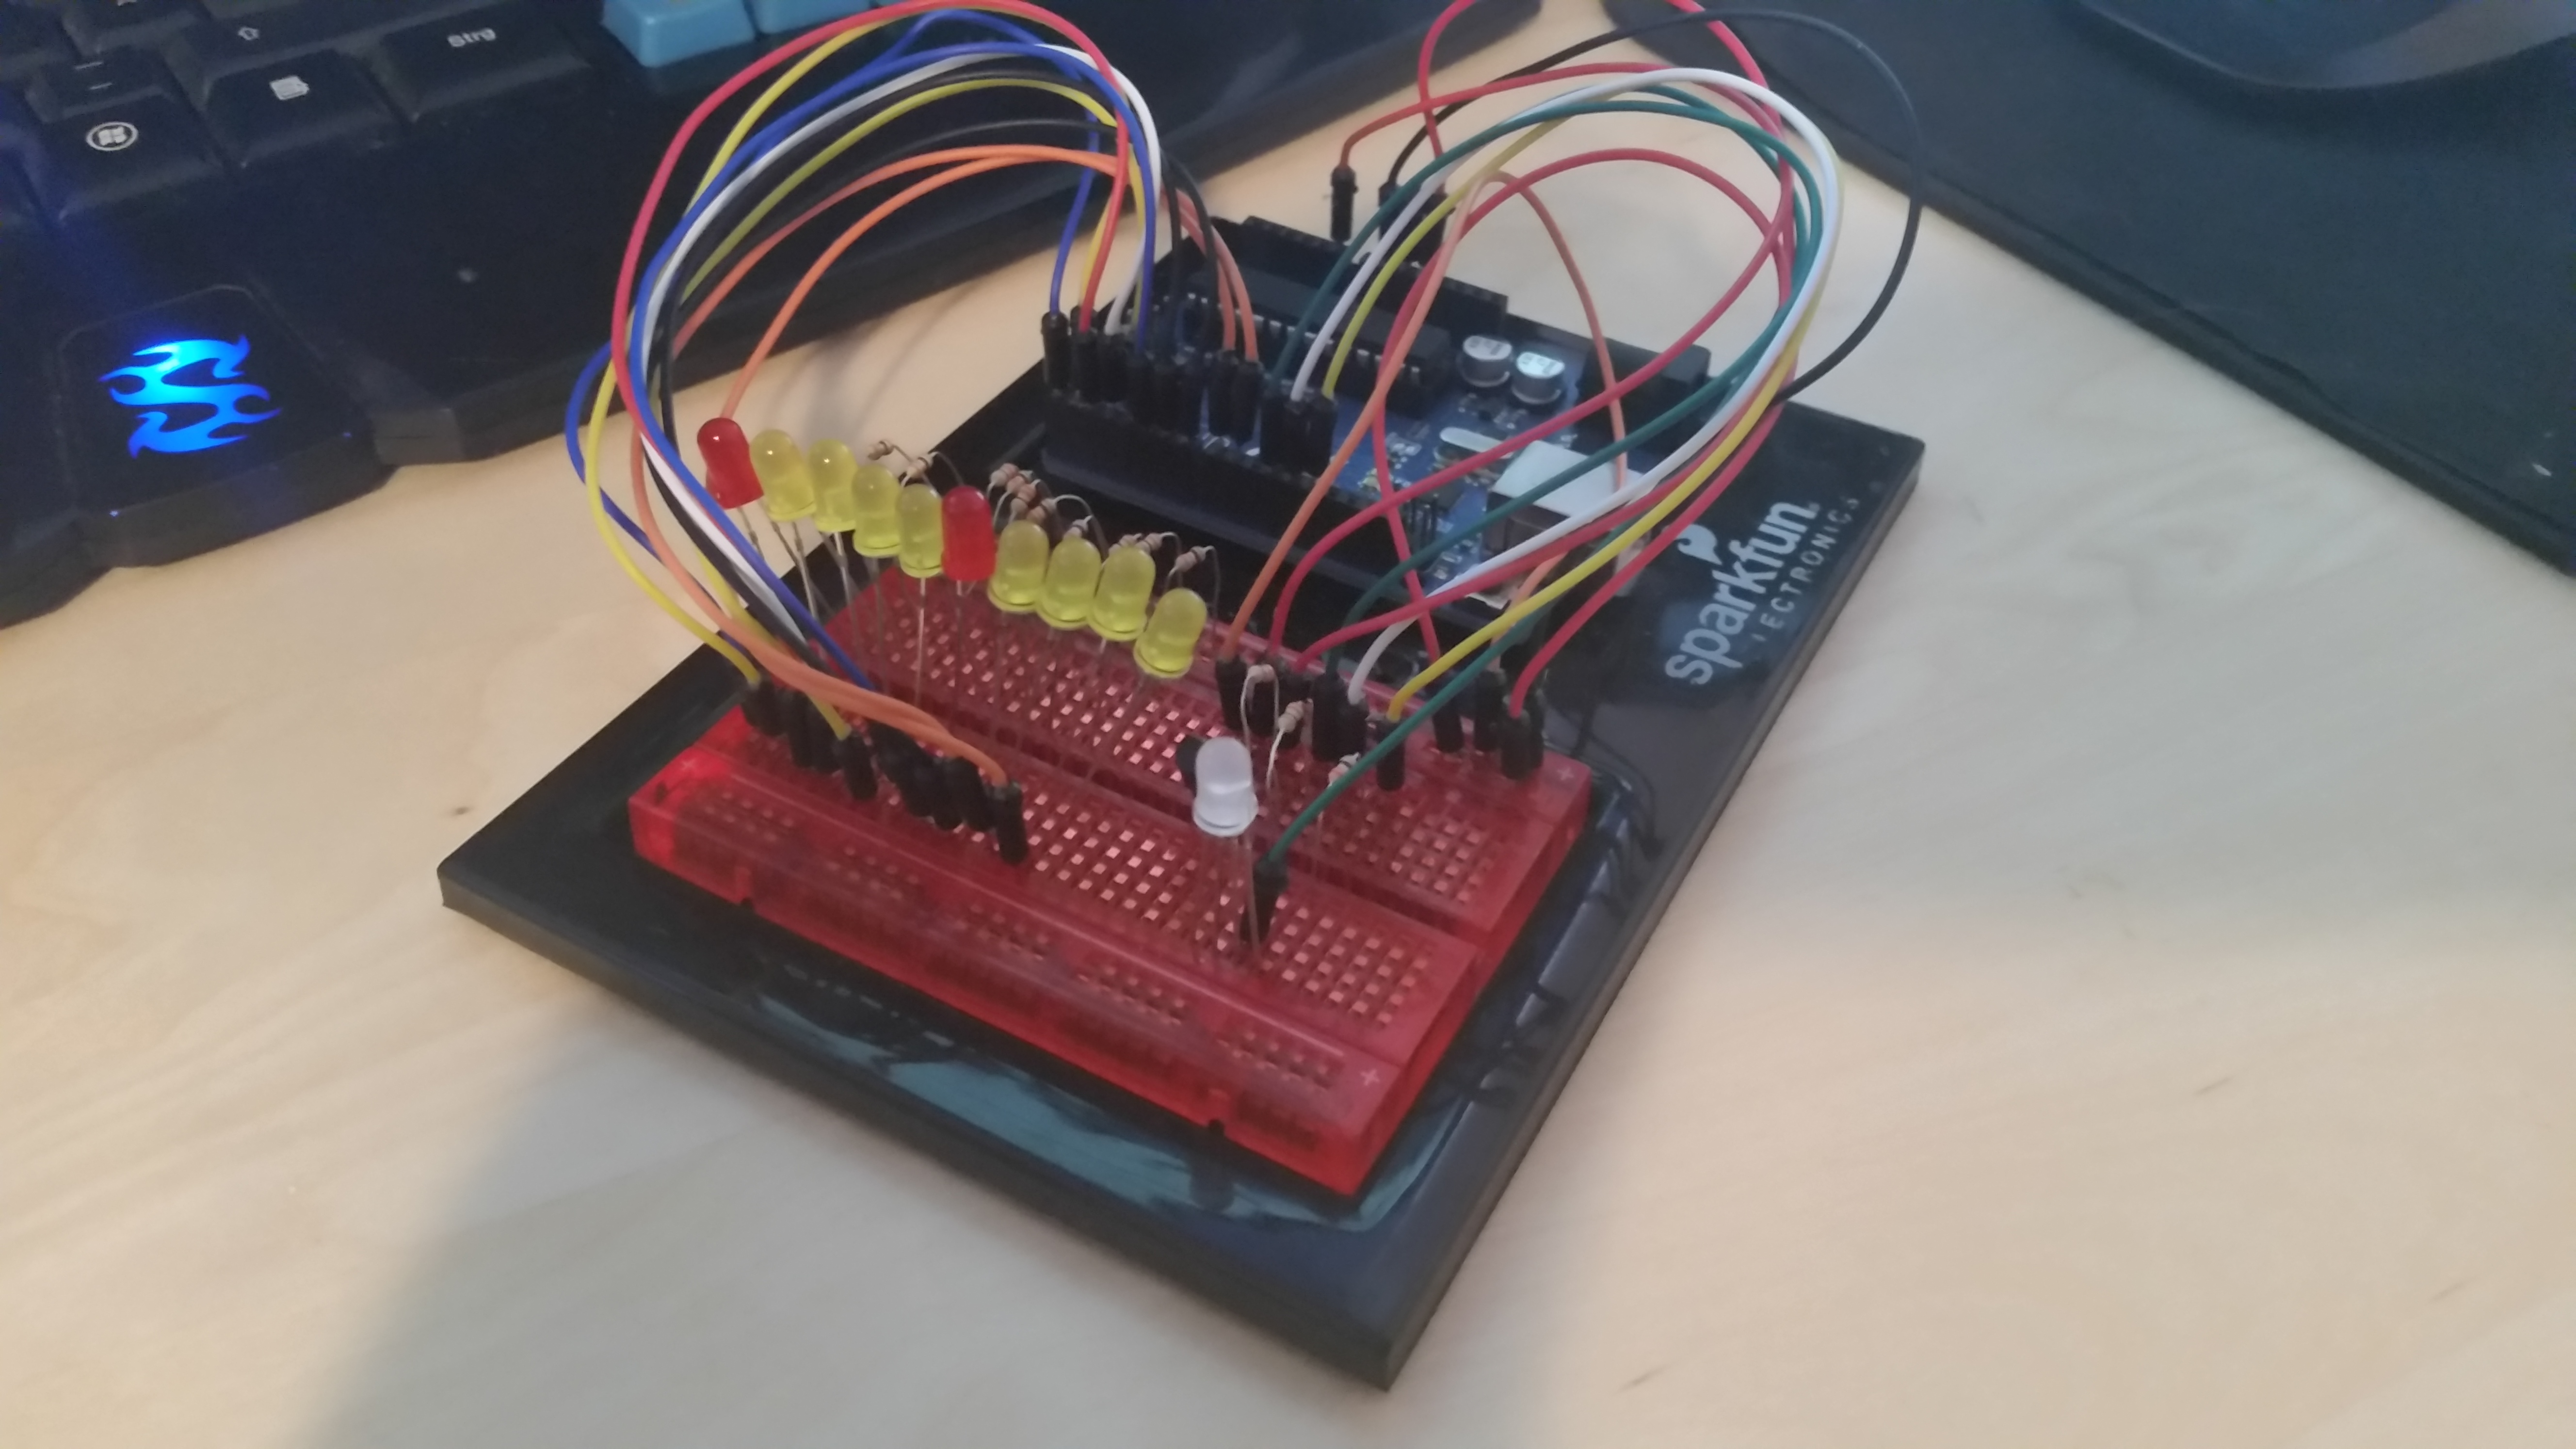
\includegraphics[height = 0.9\textheight, trim = 30cm 0cm 60cm 0cm , clip ]{../Grafiken/Aufbau_gesamt.jpg}
		\end{figure}
	\end{frame}

\end{document}
